\clearpage

\vspace{-0.25cm}
\section{Introduction}
\label{sec:introduction}

The aim of this laboratory assignment is to build an audio amplifier with the goal
of maximizing the gain and bandwidth and minimizing the total cost and the value of lower cut-off frequency.
The circuit designed has two distinct parts: the gain stage and the output stage as shown in figure \ref{fig:circuito}.

\begin{figure}[h] \centering
    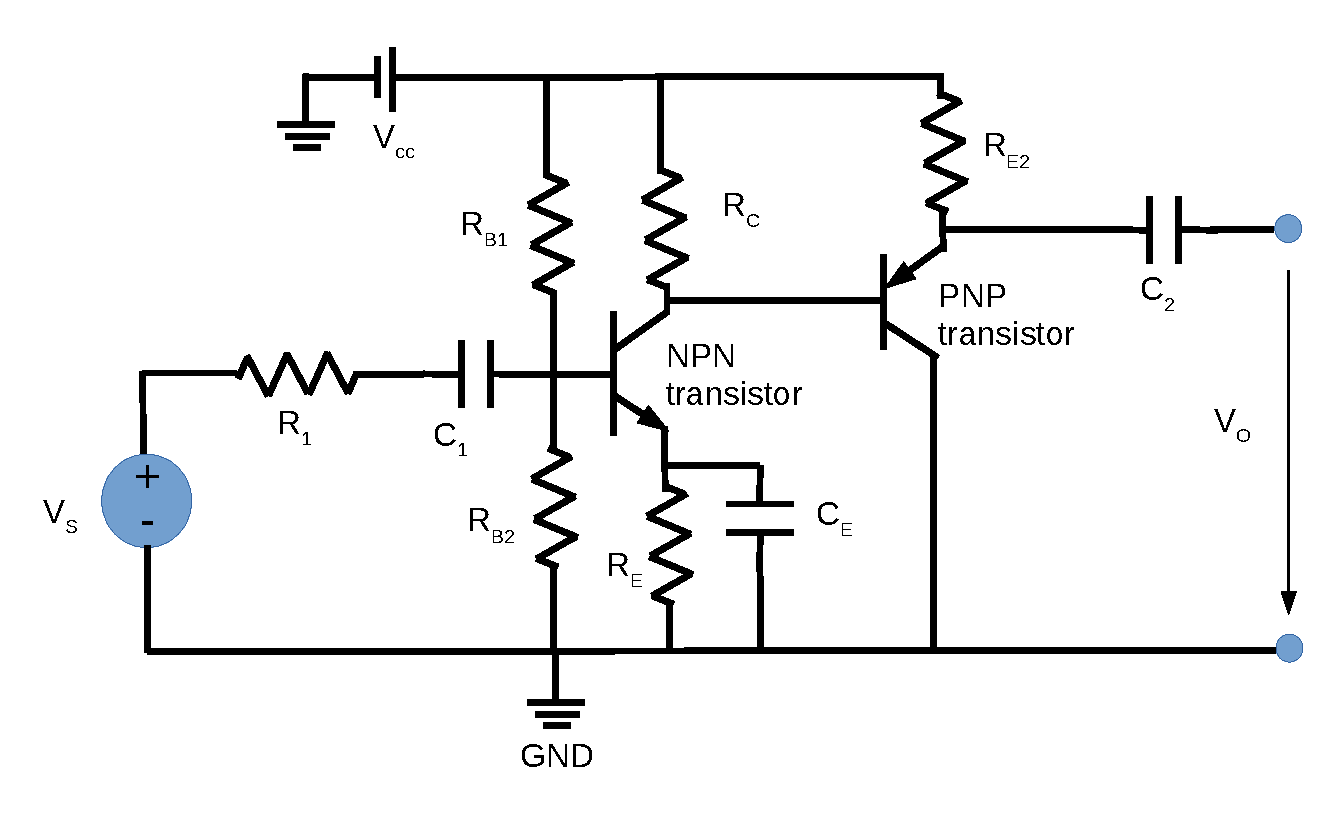
\includegraphics[scale=0.7]{lab4_principal.pdf}
    \caption{Circuit analysed.}
    \label{fig:circuito}
\end{figure}

The input ($V_{s}$) is a sinusoidal signal with a maximum amplitude of 10mV with an internal impedance of 100 $\Omega$, represented by $R_{in}$.
On the other end of the circuit we can find an 8 $\Omega$ speaker. Additionally, the circuit is supplied
by a 12V DC source, $V_{cc}$, that garantees that the transistor operates in its forward-active region (Base Biasing).

The gain stage mentioned, which is connected to the input signal, is formed by a single stage common-emitter amplifier
with degeneration that uses a NPN transistor. Furthermore, there is a bias circuit and a bypass capacitor whose
functions will be discussed soon.
Moving on to the output stage, it was used a common collector amplifier but this time a PNP transistor was used.
This stage is basically responsible for lowering the output impedance that comes from the previous stage,
so that the values are appropriate for the speaker.

Now we will talk about the goal of the coupling capacitors ($C_{1}$ and $C_{2}$), the bypass capacitor ($C_{E}$) and the effect of the resistance $R_{C}$.

Starting with $C_{1}$ and $C_{2}$, these capacitors, as well as the bias circuit, allow the transistor to operate in the forward active region. 
These capacitors block the DC component (0 V) of the source, since this DC value isn't enough to bias the transistors.
At low frequencies the impedance of coupling capacitor $C_{2}$ is relatively high and hence very small part of the signal will pass from the
amplifier stage to the load.
It is this type of changing behaviour with the frequency that explains the influence of these kind of capacitors in the cut off frequencies and, 
therefore, the bandwidth.

The bypass capacitor, $C_{E}$, blocks the DC component of the signal, where temperature stability is most important. However, in AC,
gain is most important, and this capacitor behaves like a short circuit for medium to high frequencies,
"removing" $R_{E}$ and consequently increasing the gain. 

The resistance $R_{C}$ is also important. Current $I_{C}$ influences $g_{m}$, a parameter from the transistor incremental model,
which directly influences the gain, increasing it. This way, a high $R_{C}$ is important for high gain. However, this also 
makes the output impedance high, which can make this higher gain a total waste. We need to balance the value of $R_{C}$ having this in mind.  


In Section~\ref{sec:simulation}, a theoretical analysis of the circuit is performed, followed by an simulation in \ref{sec:analysis}.
with the goal of comparing and understand better the behaviour of this circuit.

%\begin{figure}[h] \centering
%    \includegraphics[scale=0.6]{}
%    \caption{Circuit analysed.}
%    \label{fig:rc}
%\end{figure}

%\begin{figure}[h] \centering
%    \includegraphics[scale=0.4]{}
%    \caption{Positive half.}
%    \label{fig:rc2}
%\end{figure}

%\begin{figure}[h] \centering
%    \includegraphics[scale=0.4]{}
%    \caption{Negative half.}
%    \label{fig:rc3}
%\end{figure}

%\begin{figure}[h] \centering
%    \includegraphics[scale=0.75]{}
%    \caption{Wave rectified.}
%    \label{fig:rc4}
%\end{figure}

%\begin{figure}[h] \centering
%    \includegraphics[scale=0.75]{}
%    \caption{Wave rectified, with filter.}
%    \label{fig:rc5}
%\end{figure}


